Enquanto Alan e seus amigos estavam brincando, uma senhora os pediu para capinar seu lote. As crianças preferem brincar, mas, como são educadas, decidiram escolher uma das crianças para capinar o lote enquanto as outras se divertem. Para escolher quem capinará, jogarão adedanha.

Adedanha funciona da seguinte forma: todas as crianças esticam alguns dedos e o número de dedos esticados (um número de $0$ a $20$, dedos do pé também são dedos!) de cada criança são somados para um valor $S$. Depois disso conta-se \textbf{circularmente} as $N$ crianças que são numeradas de $0$ (Alan) a $N - 1$. Logo a contagem se dá na seguinte ordem: $0, 1, \ldots, N - 2, N - 1, 0, 1, \ldots$. Depois de contarmos $S$ crianças, a criança em que a contagem parou será escolhida para a árdua tarefa de capinar o lote.

Alan é muito esperto e decidiu trapacear: ele só vai decidir o número de dedos que vai esticar logo depois de ver o número que cada uma das outras crianças esticou (Alan consegue contar dedos muito rápido, as outras crianças nem percebem sua trapaça!).

Dada a sua informação privilegiada Alan quer saber, para cada criança (incluindo ele próprio), se ele consegue escolher algum número de dedos para esticar de forma que esta criança capine (se vários números de dedos esticados forem possíveis para fazer certa criança capinar, imprima o menor deles) ou caso seja impossível, -1.

\begin{figure}[H]
    \centering
    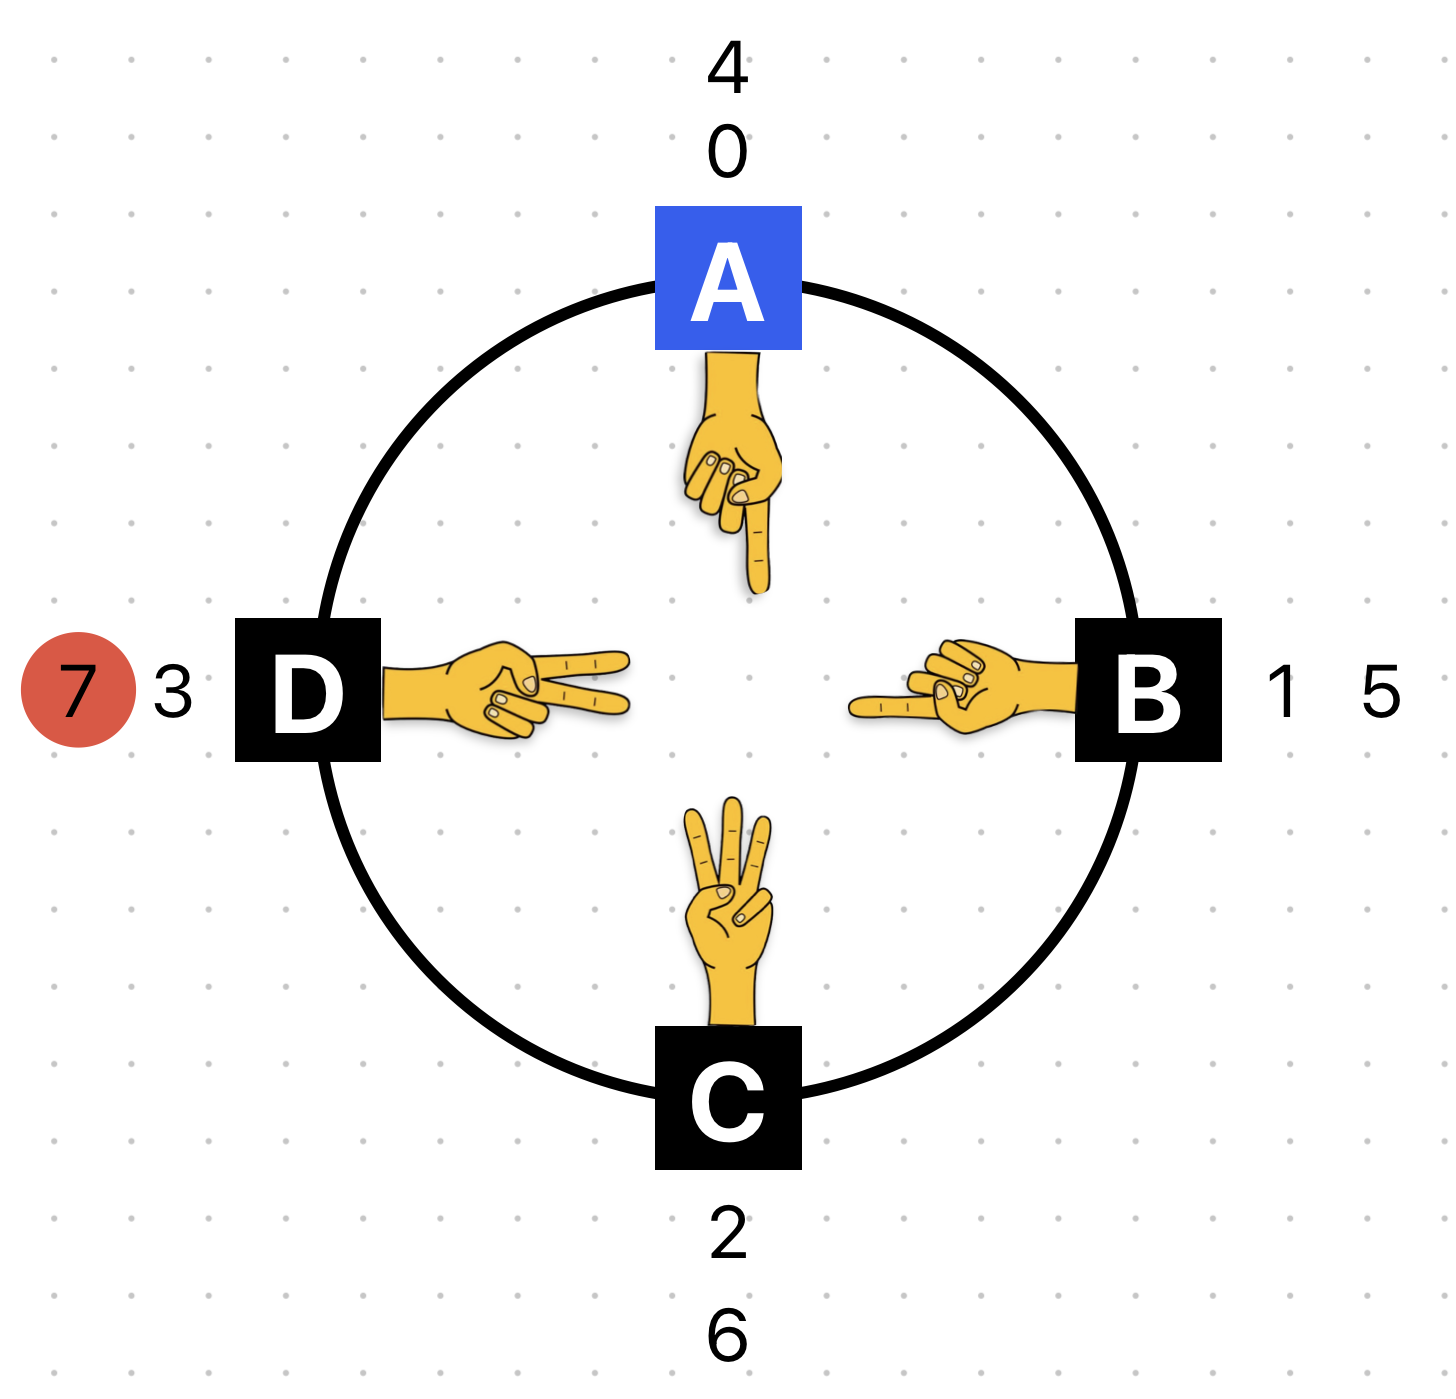
\includegraphics[width=7cm]{\CWD/adedanha.png}
    \caption{Como no Exemplo 1, se $N = 4$ e os amigos de Alan esticarem $1$, $3$ e $2$ dedos, Alan pode esticar um dedo e assim o fim da contagem caia na criança $3$ (D na figura).}
\end{figure}

\inputdesc{
A entrada contém duas linhas, a primeira contém um inteiro $N$, o número de crianças participando da adedanha (incluindo Alan).

Depois disso temos uma linha com $N - 1$ inteiros entre $0$ e $20$, o número de dedos que as crianças $1,\ldots,N - 1$ esticou (todas as crianças menos Alan). 
}

\outputdesc{
A saída deve conter $N$ números $d_0, d_1, \ldots, d_{n - 1}$. O número $d_i$ deve ser o menos número de dedos que Alan deve esticar para que a criança $i$ capine o lote e $-1$ caso seja impossível que $i$ capine.
}

\section*{Restrições}

\begin{itemize}
\item $1 \leq N \leq 10^5$
\end{itemize}

\sampleio